%
% $RCSfile: semi_structured_model.tex,v $
%
% Copyright (C) 2002-2008. Christian Heller.
%
% Permission is granted to copy, distribute and/or modify this document
% under the terms of the GNU Free Documentation License, Version 1.1 or
% any later version published by the Free Software Foundation; with no
% Invariant Sections, with no Front-Cover Texts and with no Back-Cover
% Texts. A copy of the license is included in the section entitled
% "GNU Free Documentation License".
%
% http://www.cybop.net
% - Cybernetics Oriented Programming -
%
% http://www.resmedicinae.org
% - Information in Medicine -
%
% Version: $Revision: 1.1 $ $Date: 2008-08-19 20:41:08 $ $Author: christian $
% Authors: Christian Heller <christian.heller@tuxtax.de>
%

\subsubsection{Semi Structured Model}
\label{semi_structured_model_heading}
\index{Semi Structured Model Approach}
\index{Named Values}
\index{Tagged Values}

A slightly improved version is the \emph{Semi Structured Model}. It relies on
the usage of \emph{Named Values} (sometimes called \emph{Tagged Values}), which
are stored in a dynamically extensible structure such as a list. That way,
future attributes can be added smoothly, without having to change the overall
model.

\begin{figure}[ht]
    \begin{center}
        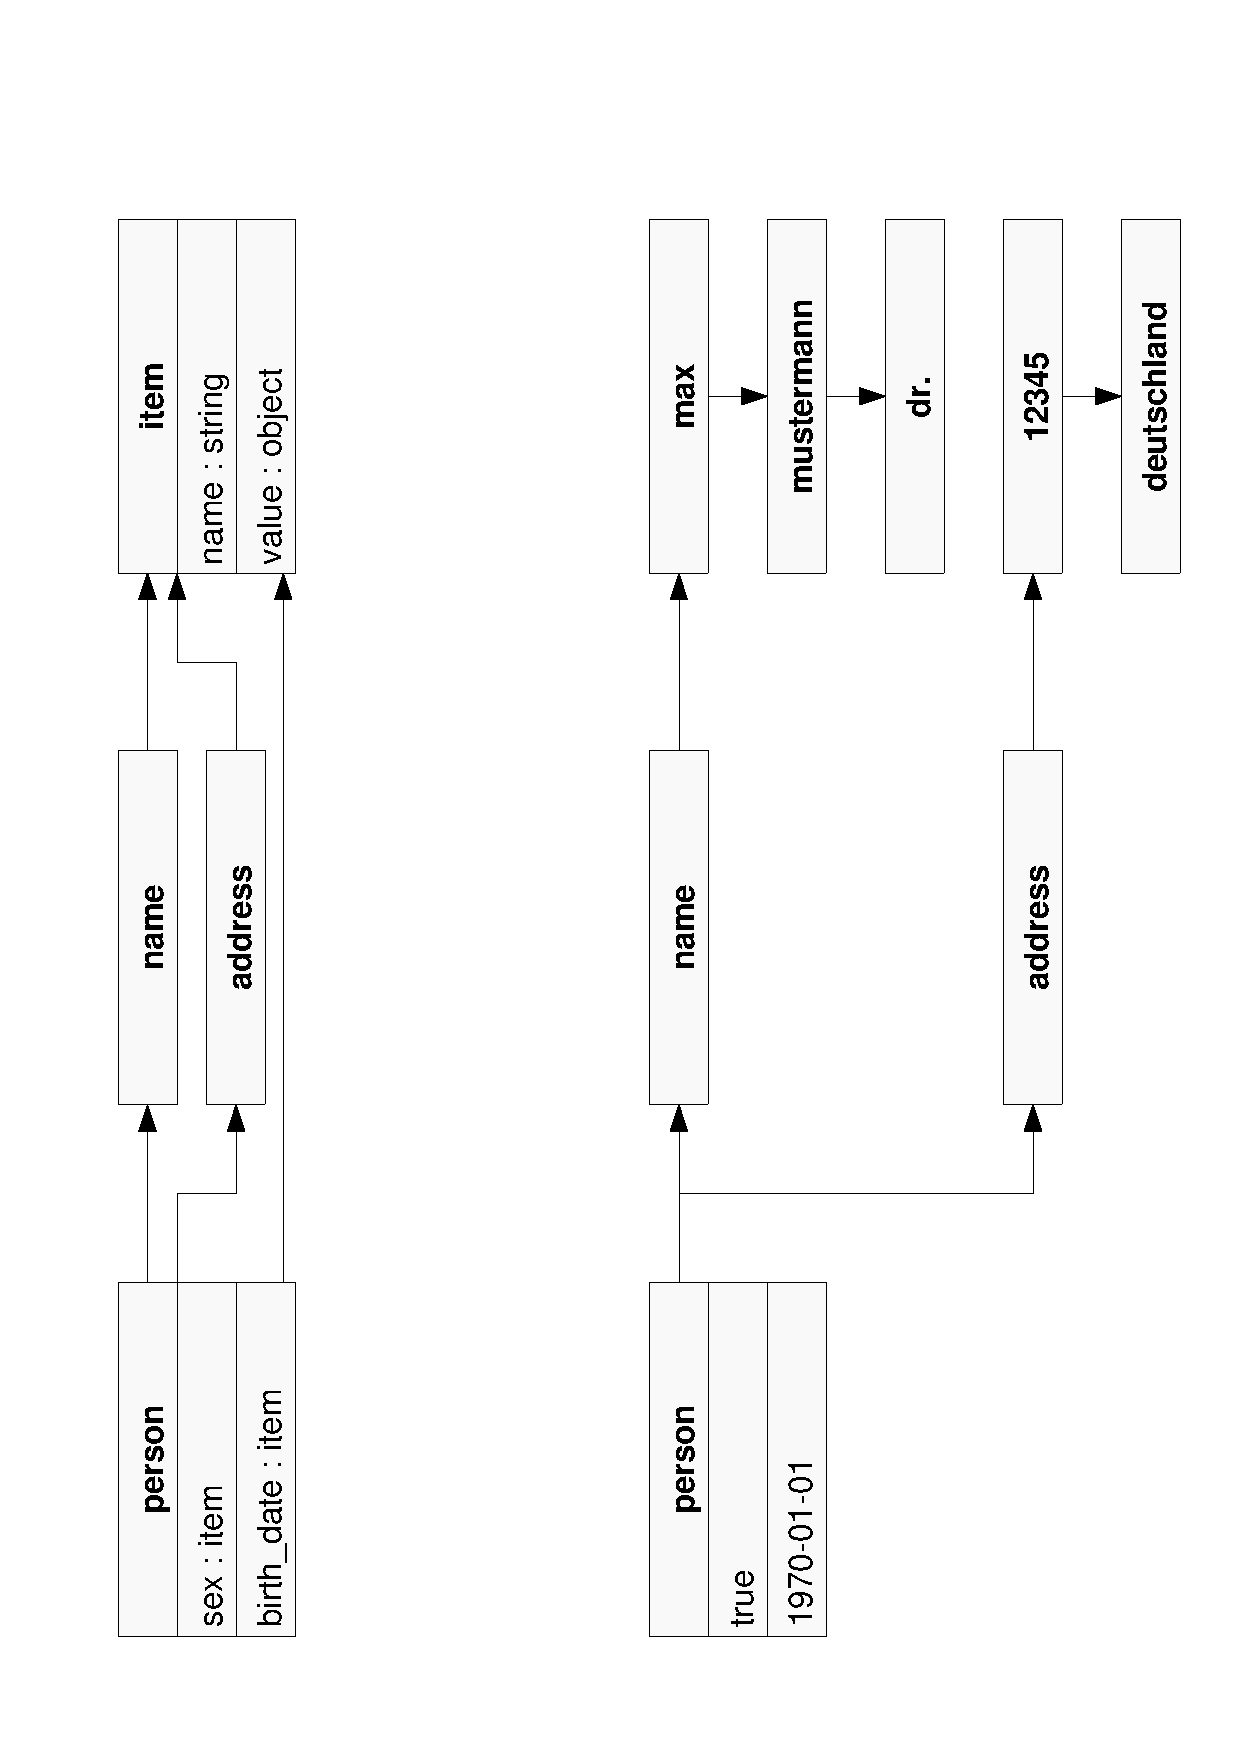
\includegraphics[scale=0.3,angle=-90]{graphic/semi.pdf}
        \caption{Semi Structured Model Approach (adapted from \cite{archetypes})}
        \label{semi_figure}
    \end{center}
\end{figure}

The example in figure \ref{semi_figure} shows a class \emph{Person} referencing
two linked lists, one called \emph{Name} and another called \emph{Address}. The
list elements are of type \emph{Item}. The dynamically extensible structure
becomes more obvious in the lower half of the figure, showing how the single
list elements reference each other. However, also here one can find
disadvantages \cite{archetypes}:

\begin{itemize}
    \item[-] Not all fields are dynamically changeable. Some are concrete
        attributes.
    \item[-] Only single lists of named values which do not allow for more
        complex internal structures are used.
    \item[-] Variability in structure is not generally dealt with.
    \item[-] Type information is lost for all list elements, since they are of
        one common type.
    \item[-] The system does not know anymore which elements are required.
\end{itemize}
